Rozwój gier wideo to złożony proces, który wymaga nieustannej uwagi i zaangażowania zespołu programistycznego. Jednym z kluczowych elementów tego procesu jest skuteczne zarządzanie i monitorowanie błędów, które mogą pojawić się podczas różnych faz produkcji. Trello, jako narzędzie do zarządzania projektami, może stanowić doskonałe wsparcie w raportowaniu i śledzeniu błędów w grze. Poniżej omówiony zostanie sposób zastosowania Trello w naszym projekcie.

\paragraph{Dev Bug List}\hspace{-1em} -- Na tej liście dodajemy karty ze zgłoszeniami błędów deweloperskich, które zostały odkryte i należy je naprawić. W karcie wybieramy etykietę \textit{Bug} oraz ewentualnie \textit{Important} jeżeli zgłoszenie ma wysoki priorytet i wybieramy kategorię, której dotyczy błąd (np.  \textit{Mechaniki} lub  \textit{Audio}). Następnie dodajemy opis, z którym musi zapoznać się deweloper jeżeli błąd jest złożony. Podpinamy się do zadania jako osoba zgłaszająca, a programista podpina się do taska samodzielnie. Wewnątrz karty z zadaniem możemy śledzić co w tym momencie dzieje się z tematem, który zgłosiliśmy poprzez zapoznanie się z komentarzami dewelopera.
\begin{figure}[h]
    \centering
    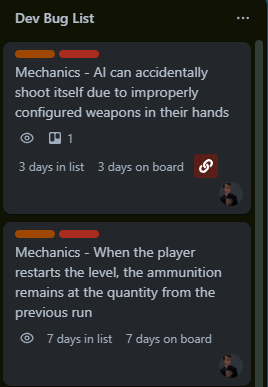
\includegraphics[scale=0.7]{Images/devBuglist.png}
    \caption{Lista rozpoznanych błędów deweloperskich występujących w grze}
    \label{fig:devBuglist}
\end{figure}
\paragraph{Visual Bug List}\hspace{-1em} -- Na tą listę trafiają zgłoszenia rozpoznanych błędów wizualnych, które należy naprawić. Podobnie jak w przypadku karty z błędami deweloperskimi w karcie wybieramy odpowiednie etykiety, dodajemy opis dla osoby, która będzie odpowiedzialna za naprawę błędu. Następnie podpinamy się do karty jako zgłaszający i czekamy aż osoba odpowiedzialna za naprawienia buga się do niej przypnie sama. Wewnątrz karty sprawdzimy postęp naprawy.
\begin{figure}[h]
    \centering
    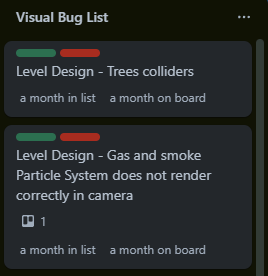
\includegraphics[scale=0.7]{Images/visBuglist.png}
    \caption{Lista rozpoznanych błędów wizualnych występujących w grze}
    \label{fig:visBuglist}
\end{figure}
\FloatBarrier
Osoba odpowiedzialna za naprawę błędu po zaznajomieniu się z zadaniem przenosi kartę do listy \textbf{Work In Progress}. \\
Po naprawie błędu osoba odpowiedzialna za niego przerzuca go do listy \textbf{Internal Test}, gdzie tester lub osoba zgłaszająca problem sprawdza czy błąd rzeczywiście udało się wyeliminować i czy przy okazji nie powstał z tego powodu inny bug:
\begin{itemize}
    \item W przypadku, gdzie problem został naprawiony i pomyślnie przeszedł testy karta z zadaniem zostaje przeniesiona do \textbf{Done} i cykl życia taska się zamyka.
    \item W przypadku, gdzie problem nie został naprawiony/powoduje innego rodzaju problemy karta z zadaniem zostaje przeniesiona do listy \textbf{Work In Progress} ze stosownym komentarzem dla osoby odpowiedzialnej za ten task (co nie zadziałało/jak odtworzyć błąd/jaka inna mechanika przestała działać po zmianach).
\end{itemize}